\documentclass{article}
\usepackage{keyval}
\usepackage{xcolor}
\usepackage{dirtree}
\usepackage{csvsimple}
\usepackage{longtable}
\usepackage{array}
\usepackage{minted}
\usemintedstyle{solarized-light}
\usepackage{tikz}
\usepackage{latex/er-diagram}%third party code from github: \usepackage{latex/er-diagram}
\usepackage[letterpaper,
	left=1.5in,
	right=0.88in,
	top=1in,
	bottom=0.89in,
]{geometry}
\usepackage{fontspec}
\usepackage[fontsize=14pt]{fontsize}
\setmainfont[Extension=.ttf,Path=fonts/timesnewroman-,UprightFont=regular,ItalicFont=italic,BoldFont=bold,BoldItalicFont=bolditalic]{}
\usepackage{calc}
\makeatletter
	%set template parameters
	\define@key{param}{title}{\newcommand\projtitle{#1}}
	\define@key{param}{name of student}{\newcommand\student{#1}}
	\define@key{param}{enrolment number}{\newcommand\enrolment{#1}}
	\define@key{param}{section}{\newcommand\room{#1}}
	\define@key{param}{class roll number}{\newcommand\roll{#1}}
	\define@key{param}{stream}{\newcommand\stream{#1}}
	\define@key{param}{name of the teachers}{\newcommand\teacher{#1}}
	%format title
	\def\@maketitle{
		\newpage\null
	\begin{center}
		{\fontsize{22pt}{\baselineskip}\selectfont\bfseries\@title }
		\par
	\end{center}
		\vspace{4\baselineskip}%skip 4 lines
	}
\makeatother
%metadata
\usepackage{hyperref}
\hypersetup{
	pdfinfo={
		Author={Aritra Ghosal},
		Title=-,
		CreationDate=-,
		Subject={Programming for Problem Solving},
		Producer=-,
		Creator=-,
	}
}
%-----------
\usepackage{graphicx}
\usepackage{ragged2e}
\newcommand{\opening}[1]{
	\setkeys{param}{#1}
	\title{\MakeUppercase{\projtitle}}
	\author{}
	\date{}
	\maketitle
	\begin{center}
		\fontsize{18pt}{\baselineskip}\selectfont
		\bfseries
		Submitted by\par
		\newline
	\end{center}
	\newline
	\textbf{Name of the Students: }\student\\
	\textbf{Enrolment number: }\enrolment\\
	\textbf{Section: }\room\\
	\textbf{Class Roll Number: }\roll\\
	\textbf{Stream: }\stream\\
	\textbf{Subject: }Programming for Problem Solving\\
	\textbf{Subject Code: }IVC101\\
	\textbf{Department: }Basic Science and Humanities\\
	\vspace{3\baselinsekip}
	\begin{center}
		\fontsize{16pt}{\baselineskip}\selectfont
		Under the supervision of\\\teacher\\
		\vspace{\baselineskip}
		\textbf{Academic Year: 2022-26}\\
		\vspace{\baselineskip}
		\fontsize{14pt}{\baselineskip}\selectfont
		\uppercase{project report submitted in partial fulfillment of the requirements for the first semester}
		
\includegraphics[width=1.32in,height=0.97in]{./instructions/IEM logo}\\
		\textbf{\uppercase{department of basic science and humanities\\institute of engineering and management, kolkata}}
		\newpage
		
\includegraphics[width=1.2in,height=0.85in]{./instructions/IEM logo}\\
		\vspace{2\baselineskip}
		\fontsize{18pt}{\baselineskip}\selectfont
		\textbf{\uppercase{certificate of recommendation}}
		\vspace{2\baselineskip}
	\end{center}
	\justify{\fontsize{18pt}{\baselineskip}We hereby recommed that the project prepared under our supervision by \student, entitled \projtitle{} be accepted in partial fulfillment of the requirements for the degree of partial fulfillment of the first semester.}
	\\[8\baselineskip]
	\fontsize{14pt}\selectfont
	\textunderscore\textunderscore\textunderscore\textunderscore\textunderscore\textunderscore\textunderscore\textunderscore\textunderscore\textunderscore\textunderscore\textunderscore\textunderscore\textunderscore\textunderscore\textunderscore\textunderscore\textunderscore\textunderscore\textunderscore\textunderscore\textunderscore\textunderscore\textunderscore\textunderscore\textunderscore\textunderscore\textunderscore\textunderscore
	\hfill
	\textunderscore\textunderscore\textunderscore\textunderscore\textunderscore\textunderscore\textunderscore\textunderscore\textunderscore\textunderscore\textunderscore\textunderscore\textunderscore\textunderscore\textunderscore\textunderscore\textunderscore\textunderscore\textunderscore\textunderscore\textunderscore\textunderscore\\
	\hspace*{2em}Head of the Department\hfill{}Project Supervisor\hspace*{1.5em}\\
	\hspace*{1em}Basic Sciences and Humanities\\
	\hspace*{4em}IEM, Kolkata\\
}
\usepackage{sectsty}
\sectionfont{\fontsize{24pt}{\baselineskip}\selectfont}
\subsectionfont{\fontsize{18pt}{\baselineskip}\selectfont}

\setlength{\parindent}{0pt}
\setmonofont[Extension=.ttf,Path=fonts/,UprightFont=CONSOLAB,NFSSFamily=codefont]{}
\begin{document}
\opening{
	title=Title of the Project,
	name of student=Aritra Ghosal,
	enrolment number=12022002018036,
	stream=C.S.B.S,
	section=F,
	class roll number=28,
	name of the teachers=\textcolor{red}{Name of the teachers}
}
\newpage
\section{Introduction}
	Python is a versatile and easy to use language often used in data manipulation. What separates Python from all other languages is its large number of use cases. Whereas Javascript is used for the web, C for systems, R for data, Python can be used for all three and many more. The following project demonstrates a model system run using mainly python.
	\subsection{Objective}
		This project attempts to model a small scale database management system utilized by an academic institution.
		The objective of this project is to learn and demonstrate several python programming concepts including:
			\begin{itemize}
				\item Using python code from other files
				\item Importing and using third party modules
				\item Reading and writing text files
				\item Managing CSV data
				\item Plotting data
				\item Building a basic user interface
				\item Utilizing concepts of Object Oriented Programming
			\end{itemize}
		This project also demonstrates general programming concepts such as ER diagrams.

	\begin{minipage}{\textwidth}
		\subsection{Organization of the Project}
			\dirtree{%
				.1 {.}. 
				.2 {code}. 
				.3 {batch.py}. 
				.3 {course.py}. 
				.3 {department.py}. 
				.3 {examination.py}. 
				.3 {main.py}. 
				.3 {student.py}. 
				.2 {databases}. 
				.3 {batch.csv}. 
				.3 {course.csv}. 
				.3 {department.csv}. 
				.3 {student.csv}. 
				.2 {fonts}. 
				.3 {CONSOLAB.TTF}. 
				.3 {timesnewroman-bold.ttf}. 
				.3 {timesnewroman-bolditalic.ttf}. 
				.3 {timesnewroman-italic.ttf}. 
				.3 {timesnewroman-regular.ttf}. 
				.2 {instructions}. 
				.3 {IEM logo.png}. 
				.3 {Project Details.docx}. 
				.3 {Project Report Template.docx}. 
				.2 {latex}.
				.3 {er-diagram.sty}.
				.3 {er.tex}.
				.3 {project.tex}.
				.3 {template.tex}.
				.2 {Makefile}. 
				.2 {outputs}. 
				.3 {output.log}. 
				.3 {\ldots{}}. 
			}\\
	\end{minipage}

		The \texttt{code} directory contains all the python code that is being executed at runtime.
		\texttt{batch.py} is a module that exports functions that operate on a batch.
		Likewise, \texttt{course.py} is a module that exports functions that operate on courses in the database.
		Same for \texttt{department.py}, which is a module that exports functions that operate on a department.
		\texttt{examination.py} exports the \texttt{Examination} class that represents an examination being held by the institution.\\
		\texttt{main.py} is a file with executive permissions which imports all of the above and runs a simple menu based command line user interface.\\

		The \texttt{databases} directory contains all the data in CSV format.\\

		The \texttt{fonts} directory contains the fonts required to compile this document.\\

		The \texttt{instructions} directory contains all of the raw material to given to build this project.\\

		The \texttt{latex} directory contains all of the \LaTeX{} code used to build the project report (this file).
		\texttt{template.tex} sets the default values necessary for the project report.
		\texttt{project.tex} contains the code that is compiled into the project report. It contains sources the outputs and diagrams along with the python code to include in the project report.\\
		\texttt{er.tex} contains the er diagram for the database and \texttt{er-diagram.sty} is a third party library used to draw the er diagram.

		The \texttt{Makefile} contains the build system for the entire project. It specifies the dependencies for each component and runs the commands to create each component. The \texttt{Makefile} also contains code that generates the databases and fills them with random data modelling the system as closely as possible. This is the centre point of the entire project, it determines the order and execution of everything else in the project.\\

		The \texttt{outputs} directory contains all of the output generated by the python code at runtime.
		The \texttt{output.log} file is generated file running the python code, it contains the entire interaction between the program and the user via the command line interface and stores it for future reference.
\section{Database Descriptions}
	Each student in the \texttt{student.csv} database has a unique ID, along with a name and a class roll number. Each student is associated with a single batch.\\
	Each batch in \texttt{batch.csv} is assigned a unique ID. They also have name and a department they fall under. Each batch has a list of courses and a list of students who appear for the courses.\\
	Each course in \texttt{course.csv} has an ID, subject name and a storage of marks obtained by each student appearing for the course.\\
	Each department in \texttt{department.csv} has an ID, name and list of batches that worked under that department.\\

\subsection{Database Samples}
	\begin{center}
		\subsubsection*{\texttt{batch.csv}}
		\begin{longtable}{|c|c|c|c|c|}
			\hline
			\textbf{Batch ID}&\textbf{Batch Name}&\textbf{Department Name}&\textbf{List of Courses}&\textbf{List of Students}\hline
			\csvreader{databases/batch.csv}{}{\csvcoli&\csvcolii&\csvcoliii&\ldots{}&\ldots{}\\\hline}
		\end{longtable}
		\subsubsection*{\texttt{course.csv}}
		\begin{longtable}{|c|c|c|}
			\hline
			\textbf{Course ID}&\textbf{Course Name}&\textbf{Marks Obtained}\hline
			\csvreader{databases/batch.csv}{}{\csvcoli&\csvcolii&\csvcoliii\\\hline}
		\end{longtable}
		\subsubsection*{\texttt{department.csv}}
		\begin{longtable}{|c|c|c|}
			\hline
			\textbf{Department ID}&\textbf{Department Name}&\textbf{List of Batches}\hline
			\csvreader{databases/department.csv}{}{\csvcoli&\csvcolii&\ldots{}\\\hline}
		\end{longtable}
		\subsubsection*{\texttt{student.csv}}
		\begin{longtable}{|c|c|c|c|}
			\hline
			\textbf{Student ID}&\textbf{Name}&\textbf{Class Roll No}&\textbf{Batch ID}\\\hline
			\csvreader{databases/student.csv}{}{\csvcoli&\csvcolii&\csvcoliii&\csvcoliv\\\hline}
		\end{longtable}
	\end{center}
\section{E-R Diagram}
	\begin{tikzpicture}[node distance=20em]
	\pic{entity={
		{student}
		{Student}{
			\begin{tabular}{l|l}
				PK&Student ID\\
				&Name\\
				&Class Roll Number\\
				FK&Batch ID\\
			\end{tabular}
		}
	}};
	\pic[right of=student]{entity={
		{batch}
		{Batch}{
			\begin{tabular}{l|l}
				PK&Batch ID\\
				&Batch Name\\
				FK&Department Name\\
				FK&List of Courses\\
				FK&List of Students\\
			\end{tabular}
		}
	}};
	\pic[below=5em of student]{entity={
		{course}
		{Course}{
			\begin{tabular}{l|l}
				PK&Course ID\\
				&Course Name\\
				&Marks Obtained\\
			\end{tabular}
		}
	}};
	\pic[below=5em of batch]{entity={
		{department}
		{Department}{
			\begin{tabular}{l|l}
				PK&Department ID\\
				&Name\\
				FK&List of Batches\\
			\end{tabular}
		}
	}};
	\draw[many-one](student)--(batch);
	\draw[many-many](student)--(course);
	\draw[many-one](student)--(department);
	\draw[many-one](batch)--(department);
	\draw[many-omany](batch)--(course);
	\draw[many-omany](department)--(course);
\end{tikzpicture}

\section{Programs}
	\begin{center}
		\subsubsection*{\texttt{main.py}}
		\inputminted[
			breaklines,
			breakanywhere=true,
			fontfamily=codefont,
			frame=lines,
		]{python}{code/main.py}
		\subsubsection*{\texttt{student.py}}
		\inputminted[
			breaklines,
			breakanywhere=true,
			fontfamily=codefont,
			frame=lines,
		]{python}{code/student.py}
		\subsubsection*{\texttt{course.py}}
		\inputminted[
			breaklines,
			breakanywhere=true,
			fontfamily=codefont,
			frame=lines,
		]{python}{code/course.py}
		\subsubsection*{\texttt{batch.py}}
		\inputminted[
			breaklines,
			breakanywhere=true,
			fontfamily=codefont,
			frame=lines,
		]{python}{code/batch.py}
		\subsubsection*{\texttt{department.py}}
		\inputminted[
			breaklines,
			breakanywhere=true,
			fontfamily=codefont,
			frame=lines,
		]{python}{code/department.py}
		\subsubsection*{\texttt{examination.py}}
		\inputminted[
			breaklines,
			breakanywhere=true,
			fontfamily=codefont,
			frame=lines,
		]{python}{code/examination.py}
	\end{center}
\section{Outputs}
	\begin{center}
		\subsubsection*{Command Line Interface}
		\VerbatimInput[
			frame=lines,
			breaklines,
			breakanywhere,
		]{outputs/output.log}
		\subsubsection*{CSE0466-report\_card.txt}
		\fontsize{10pt}{\baselineskip}\selectfont
		\VerbatimInput[
			frame=lines,
			breaklines,
			breakanywhere,
		]{outputs/CSE0466-report_card.txt}
		\fontsize{14pt}{\baselineskip}\selectfont
		\subsubsection*{Course Statistics-C006.png}
		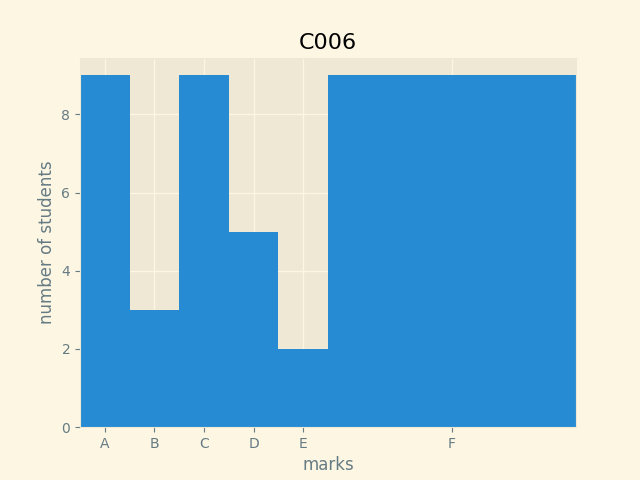
\includegraphics{outputs/Course Statistics-C006.png}
		\subsubsection*{Batch Statistics-ECE15.png}
		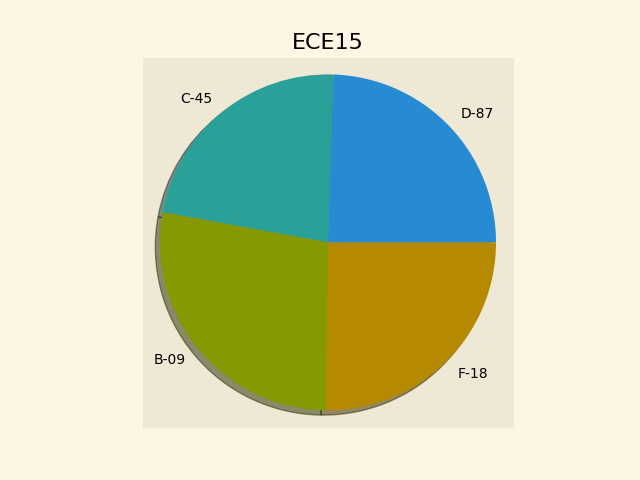
\includegraphics{outputs/Batch Statistics-ECE15.png}
		\subsubsection*{Department Statistics-CSE.png}
		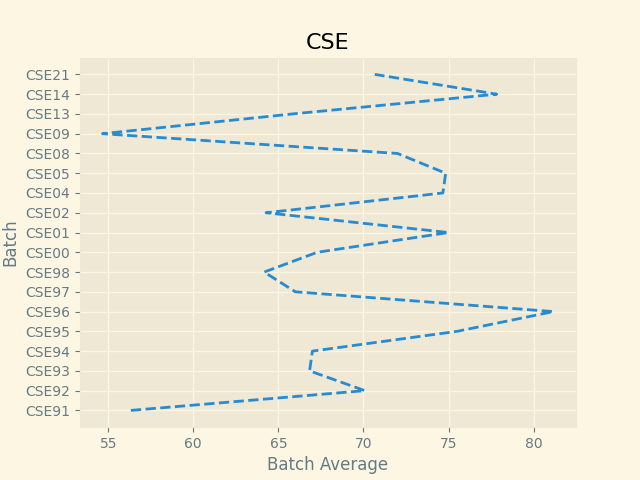
\includegraphics{outputs/Department Statistics-CSE.png}
		\subsubsection*{End Semester Exam.png}
		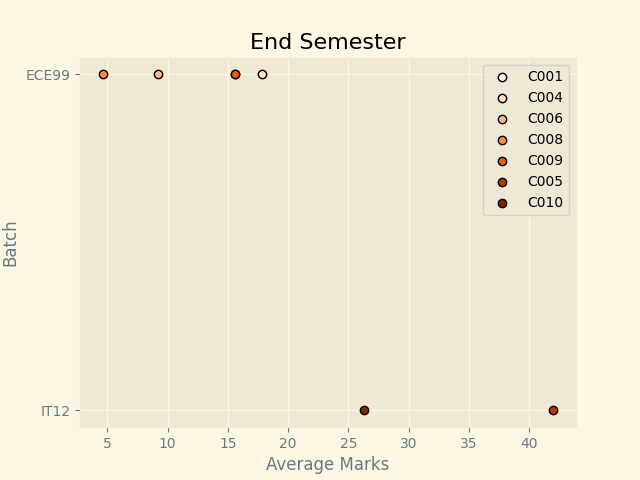
\includegraphics{outputs/End Semester Exam.png}
	\end{center}
\end{document}
